% Paper 1: when do open-source projects leave a retired LLM? (ADR 0022)
% Build from this folder with:  latexmk -pdf main.tex
% Every number comes from generated/numbers.tex (research.analysis.paper, ADR 0019).
\documentclass[pdflatex,sn-basic]{sn-jnl}

% The packages of the Springer Nature template; the class expects some of them.
\usepackage{graphicx}%
\usepackage{multirow}%
\usepackage{amsmath,amssymb,amsfonts}%
\usepackage{amsthm}%
\usepackage{mathrsfs}%
\usepackage[title]{appendix}%
\usepackage{xcolor}%
\usepackage{textcomp}%
\usepackage{manyfoot}%
\usepackage{booktabs}%
\usepackage{geometry}%
\usepackage{url}%

% Double-anonymous review: set to \anonymoustrue to hide the author and every
% link that names them (repository, Zenodo record).
\newif\ifanonymous
\anonymousfalse

\newcommand{\todo}[1]{\textcolor{red}{[TODO: #1]}}
\newcommand{\RepoURL}{\ifanonymous[anonymised]\else\url{https://github.com/imhammad/modelbump}\fi}
\newcommand{\DataDOI}{\ifanonymous[anonymised]\else\url{https://doi.org/10.5281/zenodo.23357609}\fi}
\newcommand{\RQ}[1]{\textbf{RQ#1}}
% A table from generated/tables, with its label and caption. The table is
% typeset into a box before the caption (the class's caption does not allow a
% tabular inside a box after it) and shrunk only if it is wider than the text.
\newsavebox{\gentablebox}
\newcommand{\gentable}[3]{%
  \begin{table}[t]%
  \sbox{\gentablebox}{\small\input{generated/tables/#1}}%
  \caption{#3}\label{#2}%
  \ifdim\wd\gentablebox>\textwidth
    \resizebox{\textwidth}{!}{\usebox{\gentablebox}}%
  \else
    \usebox{\gentablebox}%
  \fi
  \end{table}}

% Generated by research.analysis.paper. Do not edit: run the script again.
\newcommand{\AIAssisted}{50.7}
\newcommand{\AIAssistedGenerationDown}{42.9}
\newcommand{\AIAssistedGenerationDownHigh}{44.5}
\newcommand{\AIAssistedGenerationDownLow}{41.3}
\newcommand{\AIAssistedGenerationUp}{55.9}
\newcommand{\AIAssistedGenerationUpHigh}{56.6}
\newcommand{\AIAssistedGenerationUpLow}{55.2}
\newcommand{\AIAssistedHigh}{51.3}
\newcommand{\AIAssistedLow}{50.2}
\newcommand{\AITouchTest}{19.9}
\newcommand{\AITouchTestHigh}{26.1}
\newcommand{\AITouchTestLow}{14.9}
\newcommand{\AITouchTestOrEval}{22.5}
\newcommand{\AITouchTestOrEvalHigh}{28.9}
\newcommand{\AITouchTestOrEvalLow}{17.2}
\newcommand{\AddEval}{1.0}
\newcommand{\AddEvalHigh}{2.5}
\newcommand{\AddEvalLow}{0.4}
\newcommand{\AddTest}{7.5}
\newcommand{\AddTestHigh}{10.5}
\newcommand{\AddTestLow}{5.3}
\newcommand{\AfterAll}{57.8}
\newcommand{\AfterAllHigh}{58.7}
\newcommand{\AfterAllLow}{57.0}
\newcommand{\AfterAllTotal}{13,754}
\newcommand{\AfterFirst}{61.6}
\newcommand{\AfterFirstHigh}{62.5}
\newcommand{\AfterFirstLow}{60.7}
\newcommand{\AfterFirstTotal}{10,947}
\newcommand{\AfterGoogle}{55.7}
\newcommand{\AfterGoogleHigh}{56.4}
\newcommand{\AfterGoogleLow}{55.1}
\newcommand{\AfterGoogleTotal}{20,488}
\newcommand{\AfterLate}{62.2}
\newcommand{\AfterLateHigh}{63.1}
\newcommand{\AfterLateLow}{61.4}
\newcommand{\AfterLateTotal}{12,244}
\newcommand{\AfterWindow}{69.2}
\newcommand{\AfterWindowHigh}{70.1}
\newcommand{\AfterWindowLow}{68.4}
\newcommand{\AfterWindowTotal}{11,006}
\newcommand{\AnthropicDays}{10}
\newcommand{\AnthropicDaysHigh}{12}
\newcommand{\AnthropicDaysLow}{9}
\newcommand{\AnthropicDaysQOne}{$-$32}
\newcommand{\AnthropicDaysQThree}{77}
\newcommand{\AnthropicFirstDays}{10}
\newcommand{\AnthropicFirstDaysHigh}{12}
\newcommand{\AnthropicFirstDaysLow}{8}
\newcommand{\AnthropicFirstDaysQOne}{$-$34}
\newcommand{\AnthropicFirstDaysQThree}{77}
\newcommand{\AnthropicLateDays}{51}
\newcommand{\AnthropicLateDaysHigh}{54}
\newcommand{\AnthropicLateDaysLow}{49}
\newcommand{\AnthropicLateDaysQOne}{15}
\newcommand{\AnthropicLateDaysQThree}{115}
\newcommand{\AnthropicNoticeUsed}{52.6}
\newcommand{\AnthropicPeakShare}{24.7}
\newcommand{\AnthropicPeakShareHigh}{25.5}
\newcommand{\AnthropicPeakShareLow}{23.9}
\newcommand{\AnthropicPeakWindow}{0 to 30 days after}
\newcommand{\Candidates}{254,765}
\newcommand{\ExactDays}{11}
\newcommand{\ExactDaysHigh}{13}
\newcommand{\ExactDaysLow}{9}
\newcommand{\ExactDaysQOne}{$-$42}
\newcommand{\ExactDaysQThree}{87}
\newcommand{\ExactFirstDays}{10}
\newcommand{\ExactFirstDaysHigh}{12}
\newcommand{\ExactFirstDaysLow}{9}
\newcommand{\ExactFirstDaysQOne}{$-$43}
\newcommand{\ExactFirstDaysQThree}{87}
\newcommand{\ExactLateDays}{62}
\newcommand{\ExactLateDaysHigh}{64}
\newcommand{\ExactLateDaysLow}{59}
\newcommand{\ExactLateDaysQOne}{17}
\newcommand{\ExactLateDaysQThree}{144}
\newcommand{\ExactNoticeUsed}{50.0}
\newcommand{\ExactPeakShare}{22.3}
\newcommand{\ExactPeakShareHigh}{23.0}
\newcommand{\ExactPeakShareLow}{21.5}
\newcommand{\ExactPeakWindow}{0 to 30 days after}
\newcommand{\FailedWindows}{0}
\newcommand{\FileCheckEvalAfter}{97.0}
\newcommand{\FileCheckEvalAfterFound}{2}
\newcommand{\FileCheckEvalAfterHigh}{99.0}
\newcommand{\FileCheckEvalAfterKappa}{0.56}
\newcommand{\FileCheckEvalAfterLow}{91.5}
\newcommand{\FileCheckEvalBefore}{96.0}
\newcommand{\FileCheckEvalBeforeFound}{1}
\newcommand{\FileCheckEvalBeforeHigh}{98.4}
\newcommand{\FileCheckEvalBeforeKappa}{0.32}
\newcommand{\FileCheckEvalBeforeLow}{90.2}
\newcommand{\FileCheckEvalHandYes}{5}
\newcommand{\FileCheckRows}{100}
\newcommand{\FileCheckTestAfter}{99.0}
\newcommand{\FileCheckTestAfterFound}{18}
\newcommand{\FileCheckTestAfterHigh}{99.8}
\newcommand{\FileCheckTestAfterKappa}{0.97}
\newcommand{\FileCheckTestAfterLow}{94.6}
\newcommand{\FileCheckTestBefore}{98.0}
\newcommand{\FileCheckTestBeforeFound}{17}
\newcommand{\FileCheckTestBeforeHigh}{99.4}
\newcommand{\FileCheckTestBeforeKappa}{0.93}
\newcommand{\FileCheckTestBeforeLow}{93.0}
\newcommand{\FileCheckTestHandYes}{19}
\newcommand{\FileHandEval}{5.0}
\newcommand{\FileHandEvalHigh}{11.2}
\newcommand{\FileHandEvalLow}{2.2}
\newcommand{\FileHandTest}{19.0}
\newcommand{\FileHandTestHigh}{27.8}
\newcommand{\FileHandTestLow}{12.5}
\newcommand{\FilesFound}{399}
\newcommand{\FilesMedian}{2}
\newcommand{\FilesSample}{400}
\newcommand{\FilesSeed}{2028}
\newcommand{\FilterKappa}{0.94}
\newcommand{\FilterKappaRows}{100}
\newcommand{\FollowsExact}{21.0}
\newcommand{\FollowsExactHigh}{21.4}
\newcommand{\FollowsExactLow}{20.5}
\newcommand{\FollowsLine}{66.9}
\newcommand{\FollowsLineHigh}{67.4}
\newcommand{\FollowsLineLow}{66.4}
\newcommand{\GenerationDown}{11.3}
\newcommand{\GenerationDownHigh}{11.7}
\newcommand{\GenerationDownLow}{11.0}
\newcommand{\GenerationUp}{60.1}
\newcommand{\GenerationUpHigh}{60.6}
\newcommand{\GenerationUpLow}{59.6}
\newcommand{\GoogleDays}{10}
\newcommand{\GoogleDaysHigh}{12}
\newcommand{\GoogleDaysLow}{9}
\newcommand{\GoogleDaysQOne}{$-$52}
\newcommand{\GoogleDaysQThree}{86}
\newcommand{\GoogleFirstDays}{11}
\newcommand{\GoogleFirstDaysHigh}{13}
\newcommand{\GoogleFirstDaysLow}{10}
\newcommand{\GoogleFirstDaysQOne}{$-$52}
\newcommand{\GoogleFirstDaysQThree}{88}
\newcommand{\GoogleLateDays}{80}
\newcommand{\GoogleLateDaysHigh}{81}
\newcommand{\GoogleLateDaysLow}{79}
\newcommand{\GoogleLateDaysQOne}{35}
\newcommand{\GoogleLateDaysQThree}{113}
\newcommand{\GoogleNoticeUsed}{--}
\newcommand{\GooglePeakShare}{20.9}
\newcommand{\GooglePeakShareHigh}{21.5}
\newcommand{\GooglePeakShareLow}{20.4}
\newcommand{\GooglePeakWindow}{31 to 90 days before}
\newcommand{\IdSwap}{25.5}
\newcommand{\IdSwapHigh}{30.1}
\newcommand{\IdSwapLow}{21.3}
\newcommand{\KimAfterShutdown}{82}
\newcommand{\KimAfterShutdownHigh}{84}
\newcommand{\KimAfterShutdownLow}{79}
\newcommand{\KimCommits}{22,555}
\newcommand{\KimFileLevel}{3,931}
\newcommand{\KimMentionEval}{4.5}
\newcommand{\KimMigration}{40,483}
\newcommand{\KimMigrationWithAI}{36,048}
\newcommand{\KimRepos}{17,703}
\newcommand{\KimTouchTest}{16}
\newcommand{\MigrationsAway}{40,876}
\newcommand{\MiningEnd}{2026-10-08}
\newcommand{\MiningStart}{2023-01-01}
\newcommand{\ModelIds}{139}
\newcommand{\NotAITouchTest}{14.9}
\newcommand{\NotAITouchTestHigh}{20.4}
\newcommand{\NotAITouchTestLow}{10.7}
\newcommand{\NotAITouchTestOrEval}{15.9}
\newcommand{\NotAITouchTestOrEvalHigh}{21.4}
\newcommand{\NotAITouchTestOrEvalLow}{11.5}
\newcommand{\OpenAIDays}{14}
\newcommand{\OpenAIDaysHigh}{22}
\newcommand{\OpenAIDaysLow}{6}
\newcommand{\OpenAIDaysQOne}{$-$145}
\newcommand{\OpenAIDaysQThree}{209}
\newcommand{\OpenAIFirstDays}{11}
\newcommand{\OpenAIFirstDaysHigh}{21}
\newcommand{\OpenAIFirstDaysLow}{5}
\newcommand{\OpenAIFirstDaysQOne}{$-$145}
\newcommand{\OpenAIFirstDaysQThree}{221}
\newcommand{\OpenAILateDays}{178}
\newcommand{\OpenAILateDaysHigh}{192}
\newcommand{\OpenAILateDaysLow}{161}
\newcommand{\OpenAILateDaysQOne}{60}
\newcommand{\OpenAILateDaysQThree}{322}
\newcommand{\OpenAINoticeUsed}{39.2}
\newcommand{\OpenAIPeakShare}{19.9}
\newcommand{\OpenAIPeakShareHigh}{21.7}
\newcommand{\OpenAIPeakShareLow}{18.2}
\newcommand{\OpenAIPeakWindow}{more than 180 days before}
\newcommand{\OpenOrOther}{1.0}
\newcommand{\OpenOrOtherHigh}{1.1}
\newcommand{\OpenOrOtherLow}{0.9}
\newcommand{\OtherBigProvider}{2.2}
\newcommand{\OtherBigProviderHigh}{2.4}
\newcommand{\OtherBigProviderLow}{2.1}
\newcommand{\Precision}{84.0}
\newcommand{\PrecisionHigh}{89.9}
\newcommand{\PrecisionLow}{75.6}
\newcommand{\PrecisionRows}{100}
\newcommand{\RealMigrations}{34,300}
\newcommand{\Recall}{58.3}
\newcommand{\ResultsSeen}{851,580}
\newcommand{\RetiredBy}{2026-07-11}
\newcommand{\SameProvider}{96.7}
\newcommand{\SameProviderHigh}{96.9}
\newcommand{\SameProviderLow}{96.5}
\newcommand{\Searches}{11,003}
\newcommand{\TargetAnnounced}{2.9}
\newcommand{\TargetAnnouncedHigh}{3.0}
\newcommand{\TargetAnnouncedLow}{2.7}
\newcommand{\TargetCheck}{76.0}
\newcommand{\TargetCheckBefore}{72.2}
\newcommand{\TargetCheckBeforeHigh}{80.1}
\newcommand{\TargetCheckBeforeLow}{62.5}
\newcommand{\TargetCheckBeforeRows}{97}
\newcommand{\TargetCheckHigh}{83.5}
\newcommand{\TargetCheckLow}{66.6}
\newcommand{\TargetCheckRows}{96}
\newcommand{\TargetFound}{77.4}
\newcommand{\TargetFoundHigh}{77.8}
\newcommand{\TargetFoundLow}{77.0}
\newcommand{\TargetNamedProvider}{98.8}
\newcommand{\TargetNamedProviderHigh}{99.8}
\newcommand{\TargetNamedProviderLow}{93.3}
\newcommand{\TargetNamedRight}{90.0}
\newcommand{\TargetNamedRightHigh}{94.8}
\newcommand{\TargetNamedRightLow}{81.5}
\newcommand{\TargetNamedRows}{80}
\newcommand{\TargetOnList}{20.4}
\newcommand{\TargetOnListHigh}{20.9}
\newcommand{\TargetOnListLow}{20.0}
\newcommand{\TargetRows}{40,876}
\newcommand{\TargetShutDown}{8.9}
\newcommand{\TargetShutDownEarlier}{5.5}
\newcommand{\TargetShutDownEarlierHigh}{5.7}
\newcommand{\TargetShutDownEarlierLow}{5.2}
\newcommand{\TargetShutDownHigh}{9.2}
\newcommand{\TargetShutDownLow}{8.5}
\newcommand{\TestNamesModel}{13.0}
\newcommand{\TestNamesModelHigh}{16.7}
\newcommand{\TestNamesModelLow}{10.1}
\newcommand{\TierDown}{11.5}
\newcommand{\TierDownHigh}{11.9}
\newcommand{\TierDownLow}{11.2}
\newcommand{\TierUp}{9.5}
\newcommand{\TierUpHigh}{9.8}
\newcommand{\TierUpLow}{9.2}
\newcommand{\TouchEval}{2.8}
\newcommand{\TouchEvalHigh}{4.9}
\newcommand{\TouchEvalLow}{1.5}
\newcommand{\TouchPrompt}{1.0}
\newcommand{\TouchPromptHigh}{2.5}
\newcommand{\TouchPromptLow}{0.4}
\newcommand{\TouchTest}{17.3}
\newcommand{\TouchTestHigh}{21.3}
\newcommand{\TouchTestLow}{13.9}
\newcommand{\TouchTestOrEval}{19.0}
\newcommand{\TouchTestOrEvalHigh}{23.2}
\newcommand{\TouchTestOrEvalLow}{15.5}
\newcommand{\TruncatedWindows}{61}
\newcommand{\WithMigrationWord}{139,751}

\graphicspath{{generated/figures/}}

\raggedbottom

\begin{document}

\title[How late do projects leave retired LLMs?]{How Late Do Open-Source Projects Leave Retired LLMs? A Replication and Extension}

\ifanonymous
\author{\fnm{Anonymous} \sur{Author}}
\affil{\orgname{Anonymous}}
\else
\author*{\fnm{Hammad} \sur{Hassan}}\email{hammad.hassan@student.aiu.edu.my}
\affil*{\orgdiv{School of Computing and Informatics}, \orgname{Albukhary International University}, \orgaddress{\city{Alor Setar}, \state{Kedah}, \country{Malaysia}}}
\fi

\abstract{Providers of large language models (LLMs) retire model versions on fixed dates, and applications that still call a retired model stop working. A recent study by \citet{kim2026retires} reported that \KimAfterShutdown\% of open-source migrations away from a retired model happen only after its shutdown. We replicate and extend that study on a new dataset of \MigrationsAway{} commits from public GitHub repositories that move away from one of \ModelIds{} retired OpenAI, Anthropic and Google model IDs, with a migration label whose precision we measured on a blind, stratified sample (\Precision\%, 95\% CI \PrecisionLow--\PrecisionHigh). For models with exact retirement dates and at least 90 days of follow-up, \AfterLate\% (95\% CI \AfterLateLow--\AfterLateHigh) of migrations come after the shutdown: the direction holds, but the share is clearly below \KimAfterShutdown\%, and Kim's own labelling rules give \AfterKimLabel\% on our data. The median migration lands \ExactDays{} days after the shutdown, the busiest window is the first month after it, and projects that miss the deadline wait longer for OpenAI models than for Anthropic ones. \FollowsLine\% of migrations with a named target follow the provider's recommended model line, yet \TargetOnList\% move to a model that is itself already scheduled for retirement. Only \TouchTest\% of sampled migration commits touch a test file, in line with Kim's \KimTouchTest\%, and \TouchEval\% touch an evaluation file. The results hold when commits are grouped by repository, when other labels are used, and when search gaps are weighted back in. We release the dataset and the code.
}

\keywords{large language models, model deprecation, software migration, mining software repositories, replication, empirical study}

\maketitle

\section{Introduction}\label{sec:intro}

Applications that use a hosted large language model (LLM) call it by a model ID, such as \texttt{gpt-4-0613} or \texttt{claude-3-5-sonnet-20241022}. Each provider retires its model versions on a published schedule: it announces a deprecation, names a replacement, and after a notice period the model ID stops answering. An application that has not moved to another model by then fails. Unlike a deprecated library, which keeps working at the version a project pinned, a retired model leaves no version to stay on. Every project that depends on one has to migrate.

\citet{kim2026retires} gave the first large picture of how open-source projects react. Mining GitHub commits that move away from retired models, the study reports that \KimAfterShutdown\% (95\% CI \KimAfterShutdownLow--\KimAfterShutdownHigh) of migrations happen only after the shutdown, that is, after the application has already broken, and that \KimTouchTest\% of migrations touch a test file. If projects really react mostly after their software stops working, deprecation notices are not doing their job, and both providers and tool builders should change course. A finding with such consequences deserves an independent check.

This paper replicates the timing result on a newly built dataset and extends it with three questions the original study leaves open. We ask:

\begin{itemize}
\item \RQ{1} \emph{What share of migrations away from a retired model happen after its shutdown?} We repeat Kim's headline measure under several definitions, next to Kim's \KimAfterShutdown\%.
\item \RQ{2} \emph{How long before or after the shutdown do projects migrate?} A share hides whether late migrations come a day or a year late, and how much of the notice period projects use.
\item \RQ{3} \emph{What do projects migrate to?} We check whether they follow the provider's recommended replacement, stay with the same provider, or move to a model that is itself on its way out.
\item \RQ{4} \emph{Do migration commits change tests or evaluations?} Changing the model changes the behaviour of the application \citep{chen2024chatgpt,ma2024prompt}, so we look at whether the commit that switches the model also touches the code that would catch a regression.
\end{itemize}

We searched GitHub for every commit that names one of \ModelIds{} retired model IDs from OpenAI, Anthropic and Google between \MiningStart{} and \MiningEnd, which gave \Candidates{} candidate commits. A rule-based label keeps the \MigrationsAway{} commits whose message moves away from a retired model. We measured its precision on a blind, stratified sample labelled by hand (\Precision\%, 95\% CI \PrecisionLow--\PrecisionHigh), with an independent second rater ($\kappa = \FilterKappa$).

Our main findings are:
\begin{itemize}
\item The direction of Kim's result holds but its size does not. For models with exact dates and at least 90 days of follow-up, \AfterLate\% of migrations come after the shutdown (95\% CI \AfterLateLow--\AfterLateHigh). Applying Kim's own labelling rules to our data gives \AfterKimLabel\%, so the gap does not come from our label.
\item The typical migration is late by days, not months. The median lands \ExactDays{} days after the shutdown (95\% CI \ExactDaysLow{} to \ExactDaysHigh), and the busiest window is the first month after it. Projects that miss the deadline wait longer for OpenAI models than for Anthropic ones.
\item \FollowsLine\% of migrations with a named target follow the provider's recommended model line, and \SameProvider\% stay with the same provider, but \TargetOnList\% move to a model that is already on a retirement list.
\item \TouchTest\% of sampled migration commits touch a test file, which replicates Kim's \KimTouchTest\%, and only \TouchEval\% touch an evaluation file. About a quarter only swap the model ID.
\end{itemize}

The contributions of this paper are a replication of the main timing result with a measured label, three research questions that extend it, a set of robustness checks that answer the objections a reviewer would raise, and an open dataset of LLM migration commits with its validation samples (see the data availability statement).

The rest of the paper is organised as follows. Section~\ref{sec:background} describes how providers retire models and the work this study builds on. Section~\ref{sec:method} explains how the dataset was built and checked. Section~\ref{sec:results} answers the four research questions, and Section~\ref{sec:robustness} tests the timing results against alternative choices. Section~\ref{sec:discussion} discusses what the results mean, Section~\ref{sec:threats} the threats to validity, and Section~\ref{sec:conclusion} concludes.

\section{Background and Related Work}\label{sec:background}

\subsection{How providers retire models}

OpenAI, Anthropic and Google each publish a deprecation page that lists retired and retiring model IDs. For each model, OpenAI and Anthropic give the day the deprecation was announced, the day the model stops answering (the \emph{shutdown}), and a recommended replacement. Google's page gives no announcement day and, for many models, only the earliest day on which the model may be shut down. Providers sometimes postpone a retirement; we count from the earliest announcement. A model can also have several IDs, such as a dated ID and an alias that points to it.

\subsection{Deprecation and breaking changes}

How clients react when an API they use is deprecated or changed is well studied. \citet{robbes2012deprecation} followed 577 deprecated methods and 186 deprecated classes through the Squeak and Pharo ecosystems and measured how often, how widely and how quickly client systems adapted to them, and \citet{hora2018react} measured the reactions to 118 API changes across about 3,600 Pharo systems. \citet{sawant2018deprecation} repeated the deprecation study for more than 25,000 GitHub clients of five popular Java APIs and for the JDK, and found reactions strikingly similar to those in Smalltalk. Deprecation has since been studied for Android \citep{li2018deprecated}, for Python libraries, where library maintainers handle it poorly and so make it harder for clients to move away \citep{wang2020python}, for whole Python packages \citep{zhong2024package}, and for machine-learning libraries, whose deprecated APIs developers rarely prioritise \citep{haryono2021mlapi}. LLMs themselves often suggest deprecated library APIs when completing code \citep{wang2025llmdeprecated}.

Closest to our setting are web APIs, where the provider, not the client, decides when the old version stops working. Interviews with client developers and the history of four large web APIs show how provider-driven changes impose work on client code \citep{espinha2014webapi}, and a study of 2,224 OpenAPI specifications of 1,368 RESTful APIs found several severe problems in how they deprecate \citep{yasmin2020rest}. Breaking changes in library releases are common: about one release in three in Maven broke at least one API \citep{raemaekers2017semver}, although a later differentiated replication found that only 7.9\% of clients are affected \citep{ochoa2022breaking}; in npm, about 12\% of dependent packages were hit by a breaking change, 44\% of them in minor or patch releases \citep{venturini2023broke}. Developers break APIs mostly to add features and simplify interfaces \citep{brito2018break}.

\subsection{Migration and technical lag}

Library migration, the replacement of one library by another, has been studied at scale in Java \citep{he2021migration} and Python \citep{islam2024pymig}. Projects often keep outdated dependencies, even after a security advisory \citep{kula2018update}. \emph{Technical lag} measures how far a deployed dependency is behind the ideal version \citep{zerouali2019lag}, and it has been traced across the npm dependency network \citep{decan2018lag}. Bots such as Dependabot reduce lag, but developers often tune them to send fewer updates, and some projects drop them \citep{he2023dependabot}. Pre-trained models are becoming a new kind of dependency \citep{yasmin2025deps20}, and model reuse is common in ML-enabled systems \citep{sens2025integration}. A retired LLM is a dependency with an extreme form of lag: once the shutdown day passes, the old version does not merely lag, it stops answering, so doing nothing is not an option.

\subsection{Software built on LLM APIs}

A growing body of work studies software that calls LLMs. Developers who write prompts build mental models of how the model behaves, and these models are hard to make reliable \citep{liang2025prompts}. Only 21.9\% of prompt changes in open-source repositories are documented in their commit messages \citep{tafreshipour2025prompting}, and prompts lack the testing and linting that code gets \citep{pister2024promptset}. Developers of LLM applications ask about prompts, APIs, cost and non-deterministic outputs \citep{chen2025llmdev,chen2026openaiso}, and many such questions remain unanswered \citep{alam2024challenges}. In open-source LLM applications, integration defects are common \citep{shao2025integrated}, and model issues are the most frequent kind of reported issue \citep{cai2025llmissues}; LLM-generated code also misuses library APIs \citep{zhuo2026apimisuse}.

Models behind the same API name can change behaviour over time \citep{chen2024chatgpt}, and prompts that work on one model can get worse on its successor, which calls for regression tests specific to LLM APIs \citep{ma2024prompt}. Model updates can cause regressions in generated code \citep{abbassi2025recatcher}. Yet testing practice lags behind: in ML projects, only a small share of ML-specific properties is tested often \citep{openja2025testingml}, and student teams building LLM-powered systems relied largely on exploratory testing and prompt iteration \citep{magalhaes2025untestable}. A migration to a new model is a deliberate change of exactly this kind, and it is the moment such tests would matter most. To our knowledge, apart from the study we replicate, no study has measured how open-source projects migrate between LLM versions.

\subsection{Mining commits}

Mining GitHub has well-known perils, such as forks, personal projects and inactive repositories \citep{kalliamvakou2014perils}. Labels derived from mined data can be wrong: a third of issue reports labelled as bugs are not bugs \citep{herzig2013bug}, and about 44\% of the commit messages studied in five projects could be improved \citep{tian2022commit}. We therefore validate our label on hand-labelled samples (Section~\ref{sec:method}). Bots also commit code, and can be detected from their commits \citep{dey2020bots} and their comments \citep{golzadeh2021bots}. AI coding agents are a newer source of commits: their traces suggest that between 22\% and 29\% of the 128,018 projects in one study use them \citep{robbes2026agentic}, and bot-account lookups find only a small fraction of agent commits \citep{khosravani2026agents}. This is why we keep commits with AI-tool trailers in our main label and report the result without them separately.

\subsection{The study we replicate}

\citet{kim2026retires} mined GitHub commits that migrate away from retired LLMs and reported their timing relative to each model's deprecation and shutdown, which files they change, and how they mention evaluations. It reports \KimCommits{} migration commits from \KimRepos{} repositories, of which \KimAfterShutdown\% come after the shutdown; \KimTouchTest\% of the \KimFileLevel{} migrations with file data touch a test file (Section~4.4 of that paper), and \KimMentionEval\% of commit messages mention an evaluation or regression suite (Section~4.5). It keeps commits with a migration word, drops moves into the retired model, commits from bots, commits with an AI coding-tool trailer, and commits made more than 30 days before the deprecation notice. Our replication keeps those rules as one of its labels (Section~\ref{sec:labels}) and adds a stricter one.

\section{Study Design}\label{sec:method}

Table~\ref{tab:dataset} summarises how the dataset was built. All code is in the replication package (see the data availability statement); each step writes its counts to a file, and one script turns those files into every number, table and figure in this paper.

\subsection{Retirement registry}

We copied every retirement listed on the deprecation pages of OpenAI, Anthropic and Google into a registry: the model ID and its aliases, the announcement day, the shutdown day, the recommended replacement, and earlier plans when a retirement was postponed. For OpenAI and Anthropic the dates are exact. Google gives no announcement day and, for many models, only the earliest possible shutdown day, so we report Google separately throughout. Gemini~1.5 models, which are no longer on Google's deprecation page, are used only to tell whether a migration target was already shut down (RQ3).

\subsection{Mining candidate commits}

For each of the \ModelIds{} model IDs and aliases we ran GitHub's commit search for the exact ID between \MiningStart{} and \MiningEnd. GitHub returns at most 1,000 results per search, so each search window was split until it held fewer, down to a single day. In total we ran \Searches{} searches and saw \ResultsSeen{} results. On \TruncatedWindows{} days a single ID had more than 1,000 results and only the first 1,000 could be seen; Section~\ref{sec:robustness} shows that this does not change the results. Five IDs had more than 50,000 results in total; we searched them only from 30 days before their earliest deprecation notice, the same cut-off Kim applies. None of these five belongs to a model counted in the RQ1 headline (Section~\ref{sec:robustness}). Because GitHub's search is fuzzy, we kept only messages that contain the exact ID, dropped forks, and kept each commit once with every repository it appears in. This gave \Candidates{} candidate commits.

\subsection{Labelling migrations}\label{sec:labels}

Each candidate gets one field per rule, so any definition of a migration can be rebuilt from the same file. The rules detect a migration word (migrate, replace, switch, upgrade, remove, deprecate and similar), the direction of the message relative to the retired ID (\emph{away}, as in ``from X'', ``X to Y'', ``replace X with'', ``X is deprecated''; \emph{into}, as in ``to X'' or ``use X''; or unclear), whether the commit falls more than 30 days before the deprecation notice, dependency-bot wording, and AI coding-tool trailers. From these fields we build three labels:

\begin{itemize}
\item \texttt{migration} follows Kim's rules: a migration word, a direction other than into, not more than 30 days before the notice, not a bot, and no AI-tool trailer (\KimMigration{} commits).
\item \texttt{migration\_strict} adds that the direction must be away.
\item \texttt{migration\_away}, our main label, keeps every commit whose message moves away from a retired model and is not from a bot, whatever its wording, date or trailer (\MigrationsAway{} commits). We designed it after a first validation round, on a separate sample of 300 commits, showed that Kim's rules keep many commits that do not move away from the retired model.
\end{itemize}

\gentable{dataset}{tab:dataset}{How the dataset was built. Each line keeps the commits of the line above that pass one more rule; the last two lines are the labels.}

\subsection{Validating the label}

Because \texttt{migration\_away} was designed after looking at labelled data, we measured it on a fresh sample: 200 candidates not used before, drawn at random with a fixed seed from three strata: commits the label keeps (100), commits kept only by Kim's rules (50), and commits neither keeps (50). The labelling sheet showed only the commit and its message, never the label. The author labelled every row. An AI assistant then flagged rows that might be mislabelled, mostly commits that move into the retired model rather than away from it; the author re-checked each flagged row and made every final decision (see the declarations), and we report these final labels. A colleague independently labelled the first \FilterKappaRows{} rows from a blank copy, with no help, and agreed with $\kappa = \FilterKappa$ \citep{cohen1960}. Of the \PrecisionRows{} labelled commits the label keeps, \Precision\% are real migrations (95\% Wilson interval \PrecisionLow--\PrecisionHigh; \citealp{wilson1927}). Weighting each stratum by its size, the label finds about \Recall\% of all real migrations among the candidates. Table~\ref{tab:validation} lists every check.

\gentable{validation}{tab:validation}{Checks of the labels against hand labels. Agreement with 95\% Wilson intervals; $\kappa$ is Cohen's kappa. ``Before the fix'' is the score of the rules as they were when the sample was drawn, which is the validation result; ``after'' shows what the fix changed.}

\subsection{Placing migrations on the timeline (RQ1, RQ2)}

For each migration we take the retired model the message moves away from (if there are several, the one shut down first) and compare the commit day with that model's announcement and shutdown. A commit is \emph{after the shutdown} if it is made on or after the shutdown day. The commit day is the committer date, since GitHub search works on it.

A model shut down shortly before our data ends has had little time to collect late migrations, which would lower the share after the shutdown. Our headline therefore counts only OpenAI and Anthropic models shut down by \RetiredBy, which leaves at least 90 days of data after every shutdown, and reports the other choices next to it. For RQ2 we report the median number of days from the shutdown with a distribution-free 95\% confidence interval from order statistics \citep{conover1999}, the share of migrations in time windows around the shutdown, and, for migrations made during the notice period, how much of that period had passed.

\subsection{Finding the target model (RQ3)}

We extract the model a commit moves to from its message with eight ordered patterns, such as ``X~$\rightarrow$~Y'', ``from X to Y'', ``replace X with Y'' and ``switch to Y''. We then compare the target with the provider's recommended replacement: the exact model, a newer model of the same line (for example a newer Sonnet for a retired Sonnet), or another model. Since provider pages list what they recommend today, not on the day of the commit, the same-line measure is the fairer one and the exact match is a lower bound. We also check whether the target is itself on a retirement list, already announced for retirement, or already shut down on the day of the commit. On the hand-labelled sample the extracted target matched the hand label in \TargetCheckBefore\% of commits before we tuned the patterns on a separate, earlier sample, and in \TargetCheck\% after; when the code names a target, it names the right model in \TargetNamedRight\% of cases.

\subsection{Changed files (RQ4)}

The search results do not include changed files, so we drew a random sample of \FilesSample{} migrations (seed \FilesSeed) and fetched each commit from GitHub's API; \FilesFound{} were still available. Each changed file is sorted by its path into a kind: test, evaluation, prompt, CI, documentation, configuration, code or other. A commit \emph{touches a test} if it adds or changes a test file, and \emph{touches an evaluation} if it adds or changes an evaluation file, such as a benchmark, golden outputs or an evaluation config. A \emph{pure ID swap} changes nothing but the model ID in the lines it edits. The author checked the file kinds by hand on \FileCheckRows{} of these commits, blind to the code's answer. The rules then agreed on tests in \FileCheckTestBefore\% of commits ($\kappa = \FileCheckTestBeforeKappa$) and on evaluations in \FileCheckEvalBefore\% ($\kappa = \FileCheckEvalBeforeKappa$); the code found only \FileCheckEvalBeforeFound{} of the \FileCheckEvalHandYes{} evaluation changes seen by hand. We improved the rules from the disagreements, which raised agreement to \FileCheckTestAfter\% and \FileCheckEvalAfter\%, and we treat the evaluation share as a lower bound.

\section{Results}\label{sec:results}

\subsection{RQ1: What share of migrations come after the shutdown?}

Table~\ref{tab:timing} gives the share of migrations made on or after the shutdown day under each choice of which migrations to count. For OpenAI and Anthropic models shut down by \RetiredBy, so that every model has at least 90 days of data after its shutdown, \AfterLate\% of \AfterLateTotal{} migrations come after the shutdown (95\% CI \AfterLateLow--\AfterLateHigh). Counting every model shut down before our data ends lowers the share to \AfterAll\%, because the most recent shutdowns have had little time to collect late migrations. Counting only migrations from 30 days before the notice onwards, as Kim does, raises it to \AfterWindow\%, because it drops the projects that moved early. Counting only the first migration of each repository away from each model gives \AfterFirst\%. Google, whose shutdown days are only the earliest possible ones, gives \AfterGoogle\%.

Every variant agrees with Kim on the direction: more migrations come after the shutdown than before it. None comes close to Kim's \KimAfterShutdown\% (95\% CI \KimAfterShutdownLow--\KimAfterShutdownHigh), and the intervals do not overlap. Section~\ref{sec:robustness} shows that the gap is not caused by our label: Kim's own rules give \AfterKimLabel\% on our data.

\gentable{timing}{tab:timing}{RQ1: share of migrations made on or after the model's shutdown day, OpenAI and Anthropic unless stated. 95\% Wilson intervals.}

\begin{quote}
\textbf{Answer to RQ1.} Most migrations away from a retired model come after its shutdown, as Kim found, but the share is about \AfterLate\%, not \KimAfterShutdown\%. Between a third and two fifths of projects migrate in time.
\end{quote}

\subsection{RQ2: How long before or after the shutdown do projects migrate?}

Table~\ref{tab:lag} and Figures~\ref{fig:windows} and~\ref{fig:ecdf} show when migrations happen relative to the shutdown. For OpenAI and Anthropic, the median migration comes \ExactDays{} days after the shutdown (95\% CI \ExactDaysLow{} to \ExactDaysHigh), and half of all migrations fall between \ExactDaysQOne{} and \ExactDaysQThree{} days. The busiest window is \ExactPeakWindow{} the shutdown, with \ExactPeakShare\% of migrations. Projects that migrate during the notice period do so when, at the median, \ExactNoticeUsed\% of it has passed.

Late is mostly a little late, but not always. Among migrations made after the shutdown, the median comes \ExactLateDays{} days after it, and the two providers differ: \AnthropicLateDays{} days for Anthropic and \OpenAILateDays{} days for OpenAI. Over all migrations, OpenAI and Anthropic projects migrate at practically the same time (Cliff's $\delta$~=~\CliffAll, $p$~\CliffAllP); among late migrations, OpenAI projects wait clearly longer ($\delta$~=~\CliffLate, \CliffLateSize; Section~\ref{sec:robustness}). Google migrations come a median of \GoogleDays{} days after the earliest possible shutdown day.

\gentable{lag}{tab:lag}{RQ2: days from the shutdown (negative is before). Medians with distribution-free 95\% intervals; ``Notice used'' is the median share of the notice period that had passed, for migrations made during it. Google: from the earliest possible shutdown day.}

\begin{figure}[t]
\centering
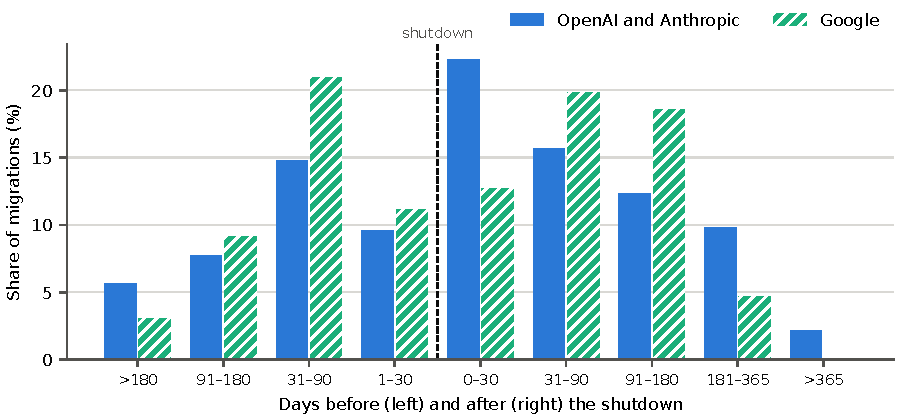
\includegraphics[width=\linewidth]{lag-windows}
\caption{RQ2: share of each provider's migrations in each time window around the shutdown.}\label{fig:windows}
\end{figure}

\begin{figure}[t]
\centering
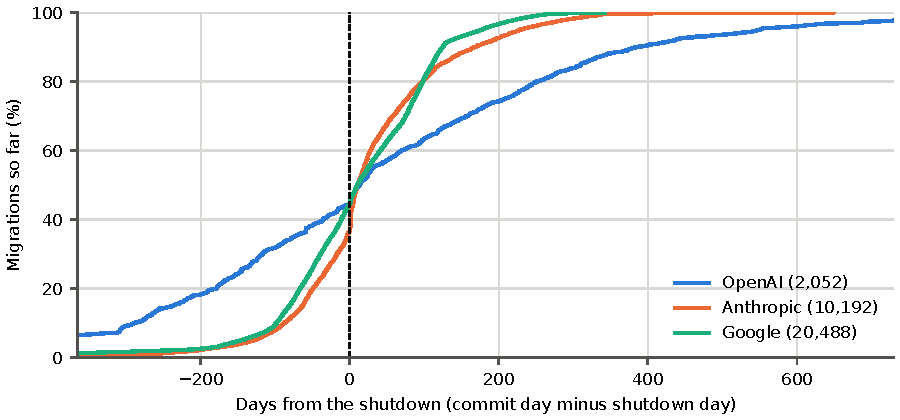
\includegraphics[width=\linewidth]{lag-ecdf}
\caption{RQ2: cumulative share of migrations by days from the shutdown, per provider.}\label{fig:ecdf}
\end{figure}

\begin{quote}
\textbf{Answer to RQ2.} The typical migration comes days after the shutdown, not months: the median is \ExactDays{} days and the busiest month is the one right after the shutdown. Projects that miss the deadline by more than that wait much longer for OpenAI models than for Anthropic ones.
\end{quote}

\subsection{RQ3: What do projects migrate to?}

\TargetFound\% of the \TargetRows{} migrations name the model they move to. Of these, \SameProvider\% stay with the same provider and only \OpenOrOther\% move to an open or other model. Table~\ref{tab:targets} and Figure~\ref{fig:targets} compare the target with the provider's recommended replacement: \FollowsExact\% move to exactly the recommended model, and \FollowsLine\% to it or another model of its line. Most targets are a newer generation of the same series (\GenerationUp\%), but \GenerationDown\% move to an older one. Table~\ref{tab:switches} lists the most common switches.

A fifth of the targets (\TargetOnList\%) are models that are themselves on a provider's retirement list today, so these projects will have to migrate again. \TargetAnnounced\% were already announced for retirement on the day of the commit, and \TargetShutDown\% had already been shut down, mostly Gemini~1.5 models (\TargetShutDownEarlier\% of all targets). \AIAssisted\% of the migrations with a target carry the mark of an AI coding tool, and they are no more likely to move to an older generation than the others.

\gentable{targets}{tab:targets}{RQ3: the target of each migration compared with the provider's recommended replacement, as a share of each provider's migrations.}

\gentable{top-switches}{tab:switches}{RQ3: the ten most common switches.}

\begin{figure}[t]
\centering
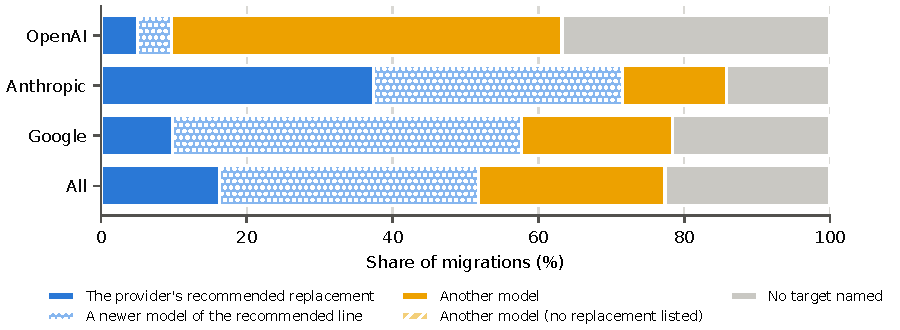
\includegraphics[width=\linewidth]{targets}
\caption{RQ3: how targets relate to the recommended replacement, per provider.}\label{fig:targets}
\end{figure}

\begin{quote}
\textbf{Answer to RQ3.} Projects almost always stay with their provider and mostly follow its recommended line, but one target in five is already scheduled for retirement.
\end{quote}

\subsection{RQ4: Do migration commits change tests or evaluations?}

Table~\ref{tab:files} and Figure~\ref{fig:files} give what the \FilesFound{} sampled migration commits change. \TouchTest\% touch a test file (95\% CI \TouchTestLow--\TouchTestHigh), which matches Kim's \KimTouchTest\%; \AddTest\% add one. Only \TouchEval\% touch an evaluation file, such as a benchmark, golden outputs or an evaluation config (\TouchEvalLow--\TouchEvalHigh). This is a lower bound: by hand we found evaluation changes in \FileHandEval\% of the checked commits. \IdSwap\% of the commits whose diffs we could read change nothing but the model ID. Commits made with an AI coding tool touch tests in \AITouchTest\% of cases and the others in \NotAITouchTest\%, but the intervals overlap.

Kim's \KimMentionEval\% for evaluations counts commit messages that mention an evaluation suite, not files, so it measures something different from our \TouchEval\%.

\gentable{changed-files}{tab:files}{RQ4: what the sampled migration commits change, with 95\% Wilson intervals.}

\begin{figure}[t]
\centering
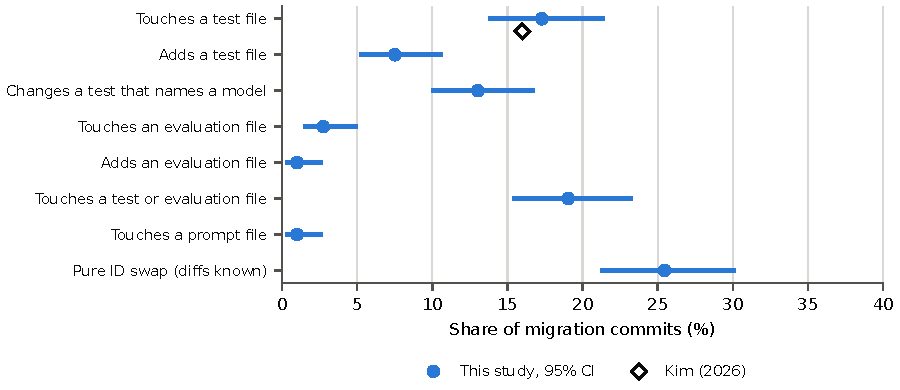
\includegraphics[width=\linewidth]{changed-files}
\caption{RQ4: shares of sampled migration commits with 95\% intervals; the diamond is Kim's \KimTouchTest\%.}\label{fig:files}
\end{figure}

\begin{quote}
\textbf{Answer to RQ4.} About one migration in six touches a test, as Kim found, and very few touch an evaluation. Most projects switch the model without changing the code that would catch a change in its behaviour.
\end{quote}

\section{Robustness of the Timing Results}\label{sec:robustness}

The answers to RQ1 and RQ2 depend on choices that a reader could question. We repeated the headline once for each such question, changing one thing at a time (Table~\ref{tab:robustness}).

\paragraph{Commits from one repository are not independent.} A repository that migrates several services at once adds several similar commits. Resampling whole repositories \citep{efron1993bootstrap}, \BootReps{} times over \BootRepos{} repositories, gives a 95\% interval of \AfterLateRepoLow--\AfterLateRepoHigh\% for the share after the shutdown and \ExactDaysRepoLow{} to \ExactDaysRepoHigh{} days for the median, which is almost the same as the per-commit intervals. Counting only the first migration of each repository away from each model gives \AfterFirst\%.

\paragraph{The label differs from Kim's.} Kim's rules (\texttt{migration}) give \AfterKimLabel\% on our data, the strict rules give \AfterStrict\%, and \texttt{migration\_away} without commits made with an AI coding tool gives \AfterNoAI\%. All of these are far from \KimAfterShutdown\%, so the difference from Kim does not come from the way we label migrations.

\paragraph{The label's mistakes may depend on timing.} If the label kept more false migrations on one side of the shutdown than the other, the share would be biased. On the hand-labelled sample, its precision is \PrecisionAfter\% for commits made after the shutdown (\PrecisionAfterLow--\PrecisionAfterHigh) and \PrecisionBefore\% for commits made before it (\PrecisionBeforeLow--\PrecisionBeforeHigh), so false migrations are more common before the shutdown. The migrations the label misses are also mostly early: \SampleMissedAfter\% of them happen after the shutdown. The two kinds of error therefore pull in opposite directions. In the sample, which covers all models, the label places \SampleLabelAfter\% of migrations after the shutdown; when each stratum is weighted by its size so that the missed migrations are counted too, the estimate for real migrations is \SampleTrueAfter\% (95\% CI \SampleTrueAfterLow--\SampleTrueAfterHigh, from resampling within strata). Because the sample is small, this check can only rule out a large bias.

\paragraph{The search may have missed commits.} On \CutDays{} days, GitHub returned only 1,000 of the results for an ID. \CutDaysBefore{} of these days fall before the model's shutdown, and together they contain only \CutRowsReweighted{} of the headline migrations. Counting each migration found on such a day as many times as the total reported by GitHub for that day divided by 1,000 leaves the share at \AfterReweighted\% (\AfterReweightedLow--\AfterReweightedHigh). The five IDs that were searched only from 30 days before their notice contribute \LateSearchedRows{} migrations to the headline, because none of their models had been shut down by \RetiredBy, except one of Google's.

\paragraph{OpenAI and Anthropic differ only by eye.} A two-sided Mann--Whitney U test \citep{mann1947}, with Cliff's $\delta$ \citep{cliff1993} as the effect size and named using the limits of \citet{romano2006}, finds no practical difference across all migrations ($\delta$~=~\CliffAll, \CliffAllSize, $p$~\CliffAllP) or across first migrations per repository ($\delta$~=~\CliffFirst, $p$~\CliffFirstP). Among migrations made after the shutdown, OpenAI projects migrate later ($\delta$~=~\CliffLate, \CliffLateSize, $p$~\CliffLateP).

\gentable{robustness}{tab:robustness}{Robustness of RQ1 and RQ2. Each line repeats the headline (OpenAI and Anthropic, models shut down by \RetiredBy) with one change. Intervals are 95\% Wilson intervals unless stated otherwise; the weighted lines use intervals from resampling repositories.}

\section{Discussion}\label{sec:discussion}

\subsection{Why our share is lower than Kim's}

Our label is not the reason: Kim's own rules give a share even lower than ours on our data (Section~\ref{sec:robustness}). The choice of which migrations to count matters more. Counting from 30 days before the notice, as Kim does, removes the projects that moved early and raises the share to \AfterWindow\%, and counting every recent shutdown lowers it to \AfterAll\%. The remaining gap may come from the set of models, the mining period and the search method, which differ between the two studies; Kim's paper is a preprint, and some of its details cannot yet be compared. The robust finding is the direction: more projects migrate after the shutdown than before it.

\subsection{Implications}

\paragraph{For developers.} The busiest moment to migrate is the month after the model has stopped answering, so many applications were probably broken for some days unless they had a fallback model. Deprecation notices give months of warning, and projects that migrate during the notice do so when, at the median, \ExactNoticeUsed\% of it has passed. A check in CI that flags model IDs with an announced retirement would turn the notice into a failing build rather than an outage. When they do migrate, projects should check the target: one in five moves to a model that is already on a retirement list.

\paragraph{For providers.} Most projects follow the recommended model line, so the recommendation is heard. Yet the share of late migrations suggests that the notice does not reach many maintainers. Notices delivered where developers look, such as warnings in API responses before the shutdown, may help more than a longer notice period.

\paragraph{For researchers and tool builders.} Only about one migration in six touches a test and very few touch an evaluation, although a new model can change behaviour in ways tests would catch \citep{ma2024prompt}. Tools that generate a behavioural regression check for the old and new model, or that make the switch with a pull request that includes such a check, address a gap that the data shows clearly. The released dataset (see the data availability statement) can serve as a benchmark for such tools.

\section{Threats to Validity}\label{sec:threats}

\paragraph{Construct validity.} A migration is identified from its commit message. The label is \Precision\% precise and finds about \Recall\% of migrations; Section~\ref{sec:robustness} shows that its errors do not change the timing result much, but they do affect every other number as well. The commit date is when the change was committed, not when it reached production, so a commit made before the shutdown may still have been deployed after it. Recommended replacements are taken from the providers' pages as they are today, not as they were on the day of each commit, so the exact match in RQ3 is a lower bound. Changes in tier and generation are based on model names, not on prices or benchmarks. Google gives only the earliest possible shutdown date, so its timing is less precise, and we never combine it with the other two providers.

\paragraph{Internal validity.} GitHub's search is fuzzy and returns no more than 1,000 results per query. We kept only messages containing the exact ID and weighted the days that hit the limit back in (Section~\ref{sec:robustness}). Five very common IDs were searched only from 30 days before their notice; none of them is in the RQ1 headline. RQ4 looks at only one commit per migration: a project may have changed its tests in another commit before or after the switch, so these shares are a lower bound for the whole migration. The evaluation share is also a lower bound for a second reason: the path rules found fewer evaluation changes than the hand check did (Section~\ref{sec:method}).

\paragraph{Conclusion validity.} Commits from the same repository are not independent; however, intervals from resampling repositories are almost the same as the per-commit ones. With thousands of commits, even small differences become statistically significant, so we report effect sizes and intervals rather than $p$-values alone.

\paragraph{External validity.} We study public GitHub repositories and three providers. Private code, other hosting platforms and other providers, including open models served by third parties, may behave differently. The period covers retirements announced up to \MiningEnd.

\paragraph{Reliability.} Every number in this paper is generated from the data by a single script, all random samples use fixed seeds, and the dataset, the hand labels and the code are publicly available (see the data availability statement).

\section{Conclusion}\label{sec:conclusion}

We replicated the finding that most open-source projects move away from a retired LLM only after it has been shut down, using \MigrationsAway{} newly mined migration commits and a measured label. The direction holds, but the share is about \AfterLate\%, not \KimAfterShutdown\%, under every definition we tried. The typical migration is a few days late; projects mostly follow the provider's recommended line but often choose a model that will soon be retired too; and few migrations include changes to tests or evaluations. The gap between a deprecation notice and the projects that depend on the model is real, and this is where tools that detect retired models and check a migration's behaviour can help.


\backmatter

\section*{Declarations}

\bmhead{Funding} The author received no funding for this work.

\bmhead{Competing interests} The author declares no competing interests.

\bmhead{Ethics approval} The study uses only public commits. The released dataset contains no commit messages, since they can contain names and email addresses; each row keeps the commit's URL instead.

\bmhead{Use of AI tools} The author used an AI assistant (Claude, by Anthropic) throughout this project. Under the author's direction it wrote most of the code that mines, filters and analyses the data, helped with the repository's documentation and Git workflow, and produced a first draft of the manuscript text, which the author revised. In the validation it read the first, earlier sample as a second rater and flagged rows in both samples that might have been mislabelled; the author re-checked every flagged row and made every final labelling decision. The study design, the hand labels and the conclusions are the author's, and the author takes full responsibility for the content of this paper.

\bmhead{Author contributions} The author designed the study, directed and checked the code, built the dataset, labelled the samples and wrote the paper with the AI assistance described above.

\bmhead{Data availability} The dataset, the hand-labelled samples and the counts behind every number are available at \DataDOI. The code that builds the dataset, this paper's numbers, tables and figures, and the paper itself is available at \RepoURL.


\bibliography{references}

\end{document}
